%not in details put in introduction

\section{Introduction}

The main goal of this research is to distinguish all dynamic objects present in the scene. The scene is observed from a camera installed in a vehicle, so called testbed.

This setup brings one big issue: non-static sensor. Thus, \textit{apriori} all the objects are moving from the sensors perspective, even the static objects, due to the motion performed by the vehicle.

The distinction between static and dynamic are considering the subjects in a global reference frame, so the goal is to be able to classify the dynamic parts in the scene using the world as reference frame. By finding the dynamic parts $O_{dynamic}$ we can perfectly obtain the static $O_{static}$ ones as well, by subtracting the dynamic one from the scene $S$.

\begin{equation}
S=O_{static}+O_{dynamic}
\end{equation}

\section{Demonstrator configuration} %configuration of the lasers, diagram
\label{sec:demonstrator}

\subsection{LIDAR laser scanners}

Our testbed is a Toyota Lexus car equipped with two LIDAR lasers scanner (Check Section~\ref{sec:testbed} for the specification) installed in the frontal bumper (Figure~\ref{fig:demonstrator:birdeye}).

\begin{figure}[h]
   \centering
     \begin{tabular}{lr}
       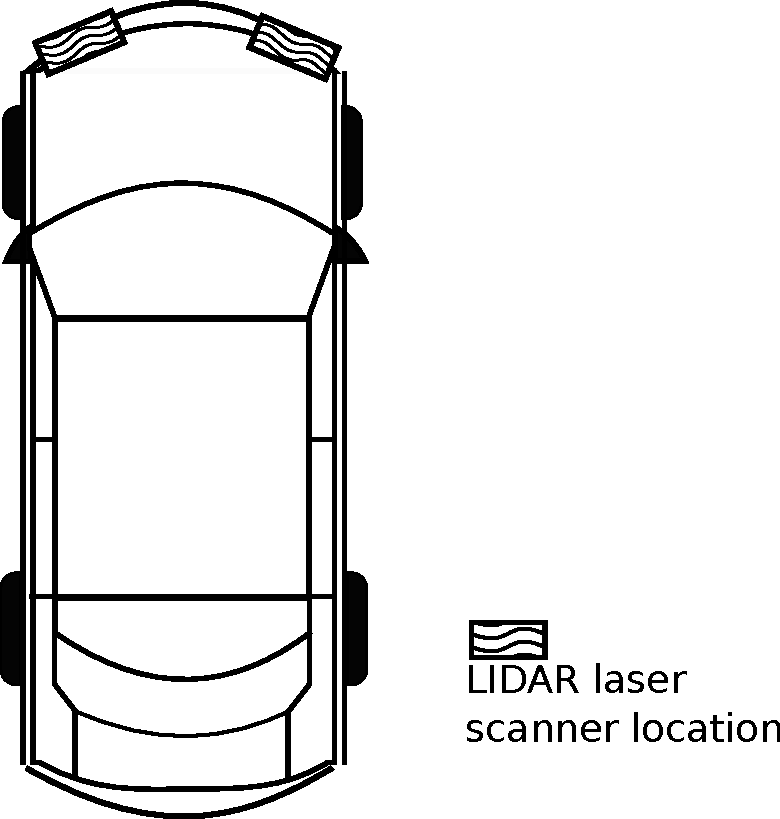
\includegraphics[scale=0.3]{img/fig:demonstrator:birdeye}
     \end{tabular}
   \caption{Bird-eye view: LIDAR laser scanners location}
   \label{fig:demonstrator:birdeye}
\end{figure}

Each LIDAR is capable of scanning in four layers, their relationship is shown  in the Figure~\ref{fig:demonstrator:lateral}, and every layers have its horizontal Field of View (FoV), one example is given for the layer 1 in the Figure~\ref{fig:demonstrator:superior}.

With four layers in total, the layers are arranged as planes with different angles but one common vetex, anchored at center of the LIDAR. The road is considered as base for the angle formation, it is formed with an imaginary plane, parallel to the road surface, and the a plane formed by the layer. Those angles are depicted in the Figure~\ref{fig:demonstrator:lateral}.

\begin{figure}[h]
   \centering
     \begin{tabular}{lr}
       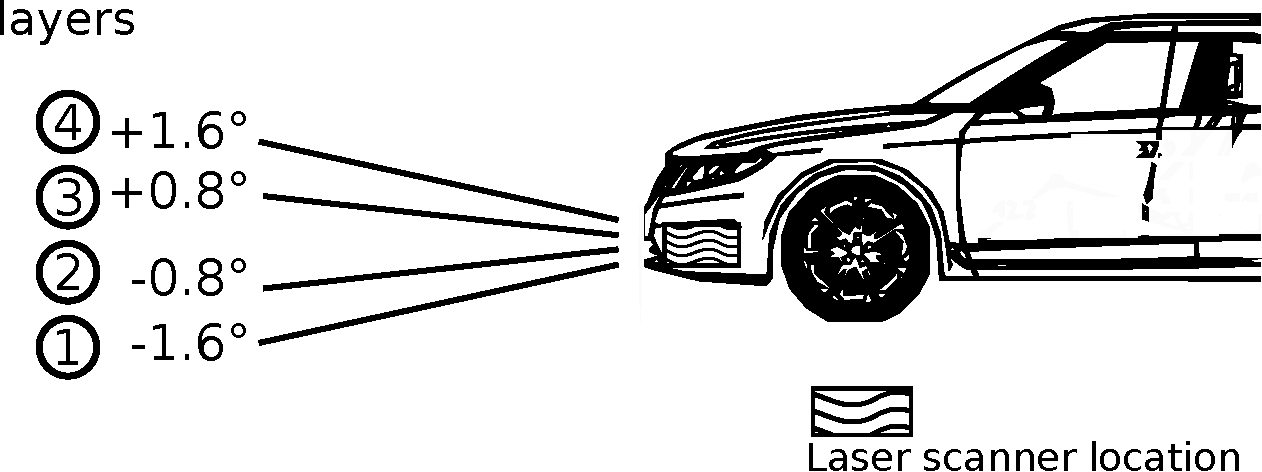
\includegraphics[scale=0.5]{img/fig:demonstrator:lateral}
     \end{tabular}
   \caption{Lateral view: Four layers of the left LIDAR laser scanner}
   \label{fig:demonstrator:lateral}
\end{figure}

A single layer sweeps the environment in a limited horizontal FoV, in the Table~\ref{tab:beam:interception} we can have the layers and their specific FoV. The LIDAR laser scanner, used in our tests, have the $0.5^{\circ}$ resolution. Meaning that every layer is capable of collecting samples at $0.5^{\circ}$ of angular distance in between. 

To calculate the number of beams available in a layer $\ell$ we apply the Equation~\ref{eq:totalbeams}, where the functions $min$ and $max$ are the minimum and maximum angles that can be reached by the layer $\ell$, and the function $resolution$ gives the resolution of the LIDAR laser scanner $\rho$, this is a specification provided by the manufacturer. 

Thus, we can calculate the number of beams in a layer based on its horizontal FoV and LIDAR resolution. Let's take as an example the first layer (layer 1) and calculate the number of beams available in this layer. 

The first layer (layer 1) has a horizontal FoV that varies from $+35^\circ$ to $-60^\circ$ (minimum and maximum FoV, respectively), the resolution of the LIDAR is $0.5^\circ$, according to the specification of the manufacturer. By applying those values in  the Equation~\ref{eq:totalbeams} we have as result $190$ beams available for the first layer.

\begin{equation}
\label{eq:totalbeams}
beams_{total}(\ell)=\frac{|max(\ell)-min(\ell)|}{resolution(\rho)}
\end{equation}

From every individual beam is possible to obtain the \textit{impact point}, meaning the distance between the LIDAR laser scanner and the first object to intercept the laser beam, limited to $200m$ maximum (More details about the specification in Section~\ref{sec:testbed}).

\begin{figure}[h]
   \centering
     \begin{tabular}{lr}
       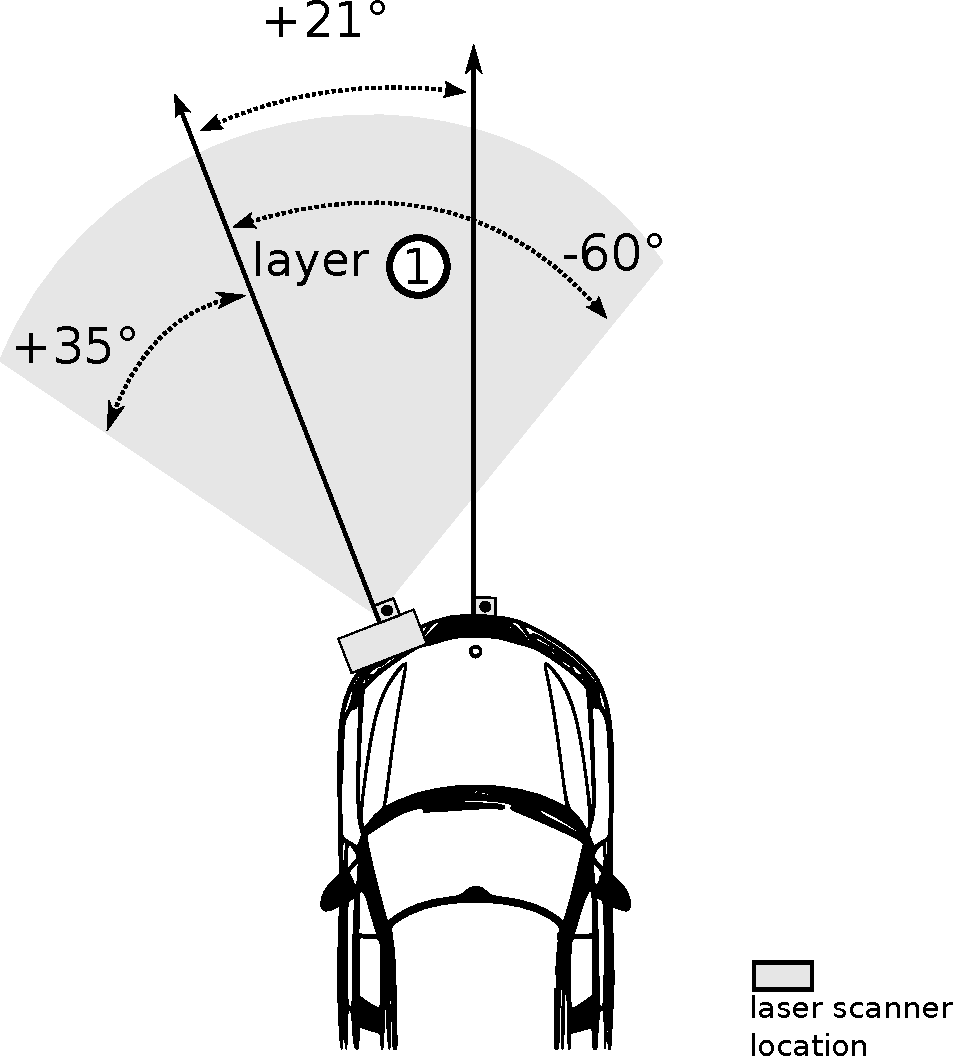
\includegraphics[scale=0.5]{img/fig:demonstrator:superior}
     \end{tabular}
   \caption{Bird-eye view: Left LIDAR laser scanner FoV, for the first layer}
   \label{fig:demonstrator:superior}
\end{figure}


\begin{table}
	\begin{center}
	    \begin{tabular}{ | c | c | c | c | c |}
		    \hline
		    Layer & $+50^\circ$ to $+35^\circ$ & $+35^\circ$ to $-50^\circ$ & $-50^\circ$ to $-60^\circ$ \\ \hline
		    4 & + & + &    \\ \hline
		    3 & + & + &    \\ \hline
		    2 &  & + & + \\ \hline
		    1 &  & + & + \\ \hline
		    $\cap$ &  & + &   \\ \hline
	    \end{tabular}
	\end{center}
    \caption{Layers and the horizontal distribution of the beams}
\label{tab:beam:interception}
\end{table}

The multiple sensor usage in the demonstrator car makes of it a complex system, due to the number of data gathered, overlapped information and possible conflicted data (Figure~\ref{fig:demonstrator:superior:overlap}). Thus, all sensor information must be carried in a consistent manner and this is accomplished by fusing the sensor information, more details about how this is done in the Section~\ref{sec:sensor:fusion}.

\begin{figure}[h]
   \centering
     \begin{tabular}{lr}
       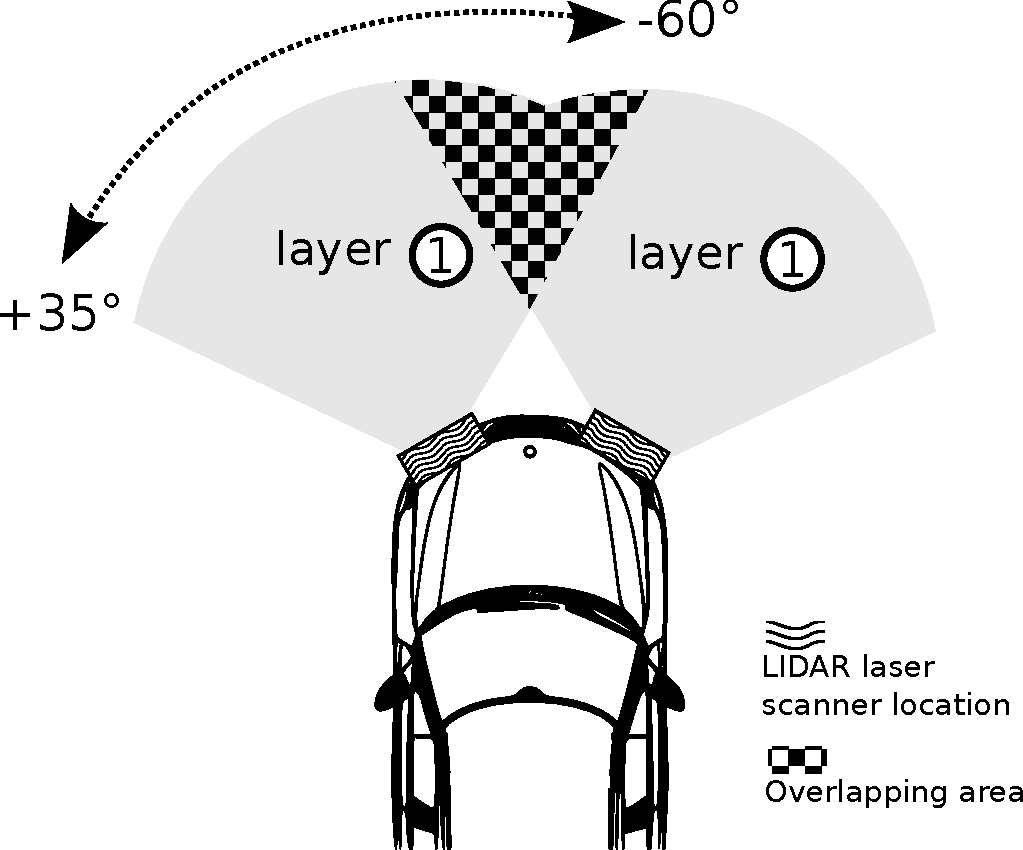
\includegraphics[scale=0.5]{img/fig:demonstrator:superior:overlap}
     \end{tabular}
   \caption{Bird-eye view: LIDAR overlapping area}
   \label{fig:demonstrator:superior:overlap}
\end{figure}

In the Figure~\ref{fig:demonstrator:superior:overlap} we depict the overlapping area when we consider the two LIDARs installed in our testbed.

\subsection{MTi-G XSens}

As we are about to see in the next Sections, the algorithm developed in this document uses two main data as input: the LIDAR data (explained previously) and MTi-G sensor data.

\begin{figure}[H]
   \centering
     \begin{tabular}{lr}
       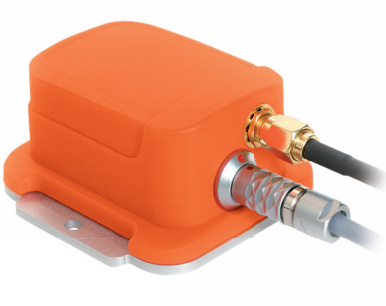
\includegraphics[scale=0.3]{img/mti-g}
     \end{tabular}
   \caption{MTi-G unit}
   \label{fig:xsens:mtig}
 \end{figure}

MTi-G unit (Figure~\ref{fig:xsens:mtig}) is a combination of Inertial Measurement Unit (IMU), GPS and barometer. The concept of MTi-G unit is not just gathering a set of sensors, it is about using information among them so that each individual sensor information can get benefits from the other ones and provide more precise information.

One example good example is that the GPS can use the other sensor to estimate the position, this is useful in case of a short-period communication outages, giving the global position estimation even without GPS signal. 

From this sensor unit our algorithm utilizes the vertical $v_y$ velocity, horizontal $v_x$ velocity and the $Yaw$ angle of the car. The $Yaw$ is the angle of the car with respect to some fix point in earth (\textit{e.g.} north oriented). The fix point is irrelevant, since we are concerned about the angle variation and not the exactly angles theirselves, as we are going to see in the Section~\ref{ch03:motiondetection}.

\section{Sensor pre-processing} %fusion module
\label{sec:sensor:fusion}

% in the last subsection, output form (occupancy grid), digrams; explains that this is our input

\subsection{Purpose}

The demonstrator car is composed with two LIDAR laser scanner sensors, as we saw in the Section~\ref{sec:sensor:fusion}. Each of the LIDAR laser scanner is composed of few layers and each layer contains several beams. Those beams are spread in a given horizontal FoV. The horizontal FoV is layer dependent, varying according to the layer.

In the Figure~\ref{fig:motion:framework}, we have represented the general framework modules for detecting the moving parts, our algorithm core is contained in the motion detection module, which will be explored later. We are making usage of two LIDARs, they provide several information from different specifications (different ranges and FoV), thus we use a fusion module which is responsible for gathering the information provided by all of the LIDAR in a consistent manner.

\begin{figure}[H]
   \centering
     \begin{tabular}{lr}
       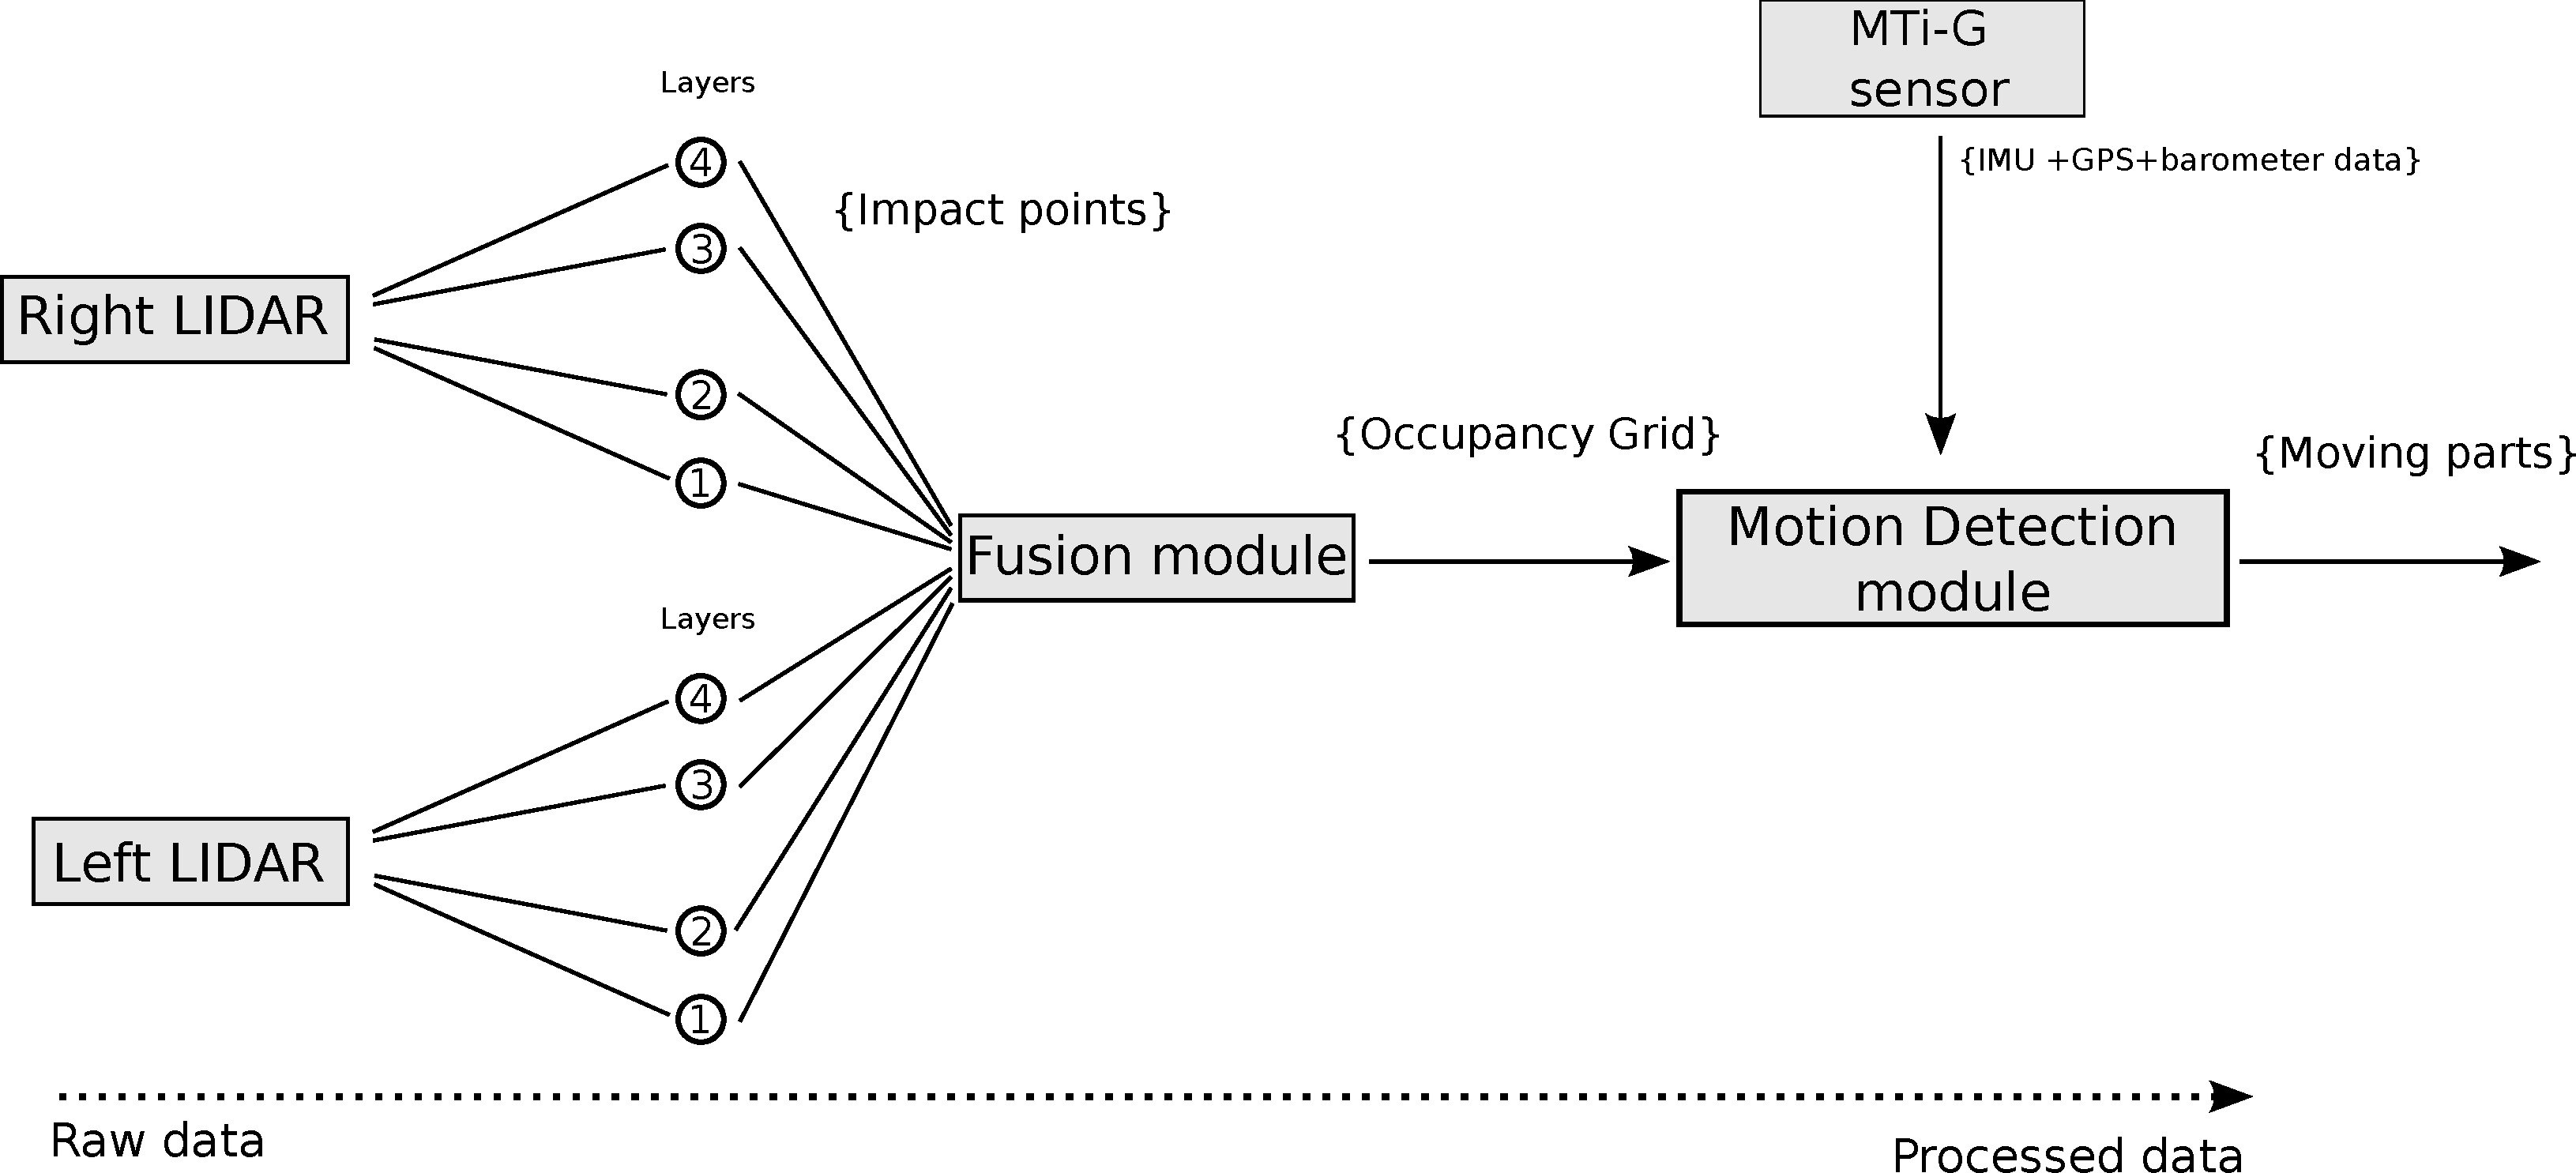
\includegraphics[scale=0.30]{img/fig:motion:framework}
     \end{tabular}
   \caption{General framework for detection of moving parts}
   \label{fig:motion:framework}
\end{figure}

This data must be gathered together, but how give a unique representation for all information provided by the sensors in one single visualization? Recall that there are overlapping scanner reading, which means that there may exist conflicting readings due to the sensor failure, or a bad environment condition.

Solving that issue implies in data fusion. \textit{Linear Opinion Pools} was used successfully by an INRIA team member to make data fusion, detailed information about this technique is explained in the document \cite{ADARVE-2012-671211}. The output of such fusing technique is an Occupancy Grid, which is used by our algorithm.

\subsection{LIDARs layers fusion}

\subsubsection{Sensor fusion from the multiple lidar layers}
Each of the  two LIDAR sensors installed on the vehicle provides us 4 layers of impact points. Each layer is used to compute an occupancy grid using the classical approach described in \cite{Thrun05}. In order to retrieve a single grid for representation of the environment, the data from all these layers are merged using the approach described in \cite{ADARVE-2012-671211}. This approach fuses the sensory information by using Linear Opinion Pools \cite{DeGroot1974}. It has the advantage of reducing the errors generated by conflicting information from the multiple layers.

The principle is to generate a posterior distribution over the occupancy of a cell $C$ of the grid given the opinion of $m$ sensors $\left\{ Y_1 \dots Y_m \right\}$.
Each sensor gives two quantities: its estimation for the occupancy of the cell $P(C | Y_i)$ and the confidence weight $w_i(C)$.
The idea is to shut-down those sensors that do not give relevant information to the process by assigning a low weight to them. The fusion of all sensory information will be as follows:

\begin{equation}
\label{linealOpinionPoolEQ}
  P(C | Y_1 \dots Y_m) = \alpha \sum \limits^m_{i=1} w_i(C) P(C | Y_i)
\end{equation}
Where $\alpha = \left[ \sum \limits^m_{i=1} w_i(C) \right]^{-1}$ is a normalization factor for the weights.  Equation \eqref{linealOpinionPoolEQ} is used to generate
2D-occupancy grids. For each sensor $Y_i$ we must define $P(C | Y_i)$, the probability of a cell being occupied given the sensor information. Complete derivations for these quantities are provided in \cite{ADARVE-2012-671211}. The output of this fusion module is an occupancy grid. %write about occupancy grid

Note that we assume independence among cells. This assumption is very strong, although it is necessary so the computation of the Equation~\eqref{linealOpinionPoolEQ} be efficient, by computing each cell value in parallel. %add section about performance

\subsubsection{Justifying the performance}

The independence among the cells is the main responsible for the high level of parallelism in the algorithm, the high level of parallelism and the performance can be assured by \textit{Amidahls law}.

\textit{Amidahls law} is a diminishing return law. It states that the gaining in performance (speedup) is not necessarily in the same magnitude as the number of new workers added for the execution of the algorithm\cite{Amdahl:1967:VSP:1465482.1465560}. This is pretty much saying that one adult female can have one children in 9 months but two adult female cannot have one children in 4.5 months, it always depends if the task can be really accomplished in parallel, of course this is an simplistic view, but gives you an idea.

In the Equation~\ref{eq:amidahls}, Amidahls describes the time to execute an algorithm in parallel ($T_p$). Its execution time depends on the time required by sequential part of the algorithm ($T_{seq}$, part which can not be parallel) along with the time for part of the algorithm that can be parallel($T_{par}$) divided by the number of workers ($p$, \textit{e.g.} number of cores in a multi-core processor).

\begin{equation}
\label{eq:amidahls}
T_p=T_{seq}+{T_{par} \over p}
\end{equation}

As in our case the cells are completely independent, the gaining in parallelization is maximum since the term $T_{seq}$ is zero (the sequential code is inexistent), and the processing time is divided among the workers.

\section{The algorithm}
%motion detection

\subsection{Principle} 

\textit{Frame} is a snapshot of the current environment representation, it is used as one of the inputs for the algorithm developed in this work.

But before jump on explanations on how the frames are going to be used, we need to describe how those frames are obtained and how do they mimic the environment.

In the Section~\ref{sec:demonstrator}, we saw that our testbed is composed by two scanners, each of them containing several layers. Every layer has a certain number of beams, which are distributed in the horizontal FoV within a regular angle interval. 

So, before having a frame that can be used by our algorithm, it is required to perform the fusion of the layers from the LIDAR, which is done by the \textbf{fusion module}. 

The details about the techniques adopted and the data processing were explained in the Section~\ref{sec:sensor:fusion}. From here on, we are going to proceed with explanation of our methods, which is identified as \textbf{motion detection module}. This module is located at the end of the processing chain, as exhibit in the Figure~\ref{fig:motion:framework}. 

\begin{figure}[h]
   \centering
     \begin{tabular}{lr}
       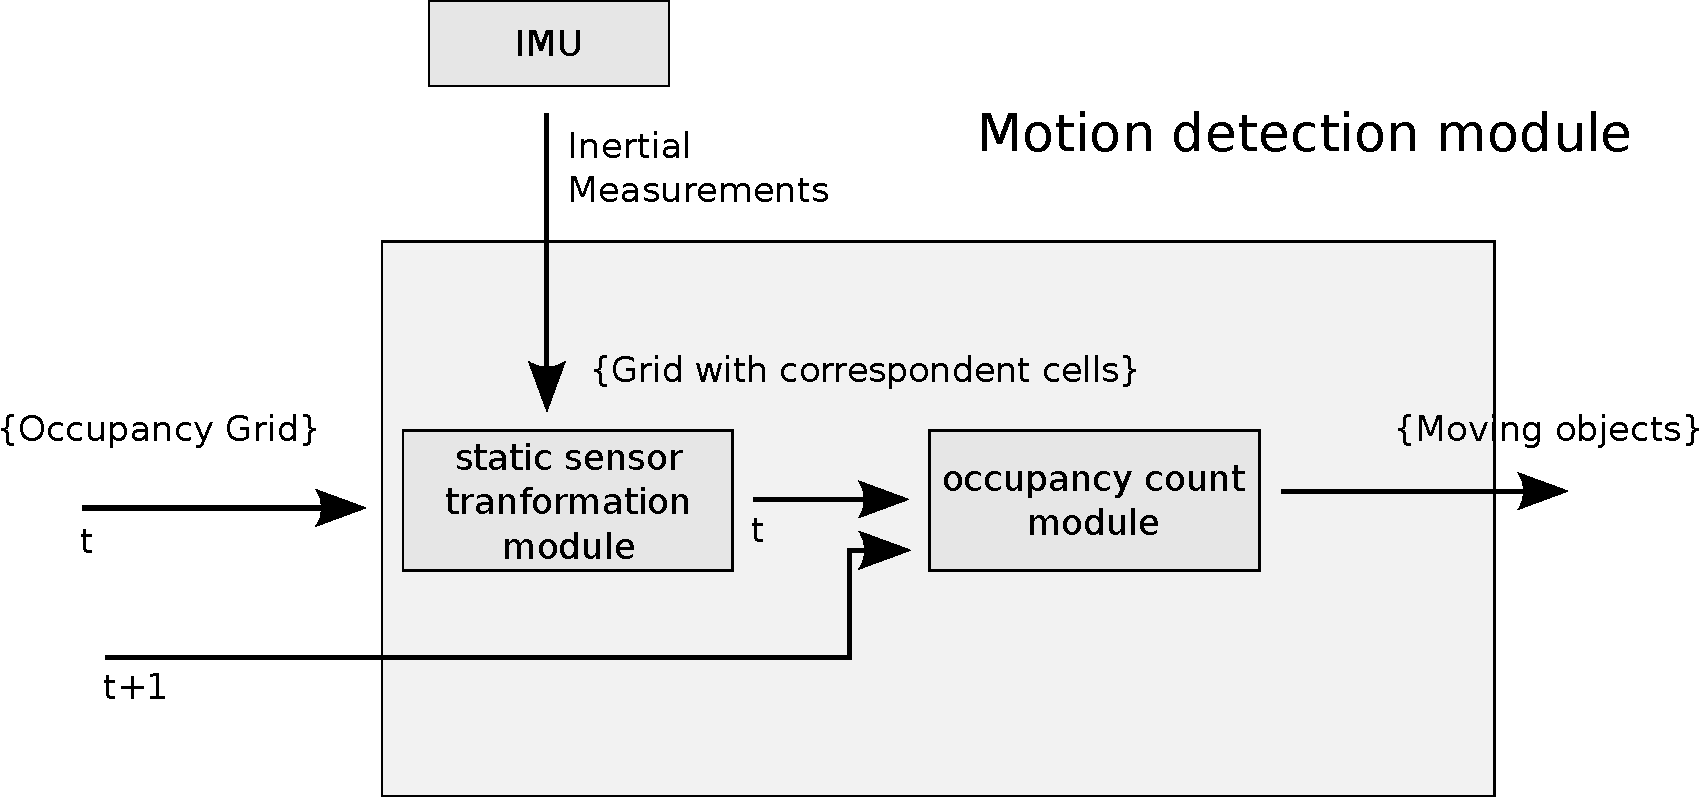
\includegraphics[scale=0.50]{img/fig:motion:framework:motionmodule}
     \end{tabular}
   \caption{Motion detection module anatomy}
   \label{fig:motion:framework:motionmodule}
\end{figure}

%%%%%%%%%%%%%%%%%%%%%%%%%%%%

\subsection{Non-static sensor issue}

The LIDAR is installed on a vehicle, the goal is to acquire measures while vehicle is moving. So it captures the surrounding and the data is processed by the \textbf{fusion module} resulting in Occupancy Grid $OG_t$. This process is repeated for each frame obtained. This is required to transform the data into the proper input for \textbf{motion detection module}.

The position of the LIDAR gives us the fully dynamic scenario impression. Meaning that, by the LIDAR sensor perspective the entire scenario is moving and all subjects are changing their position, except for those who are following the same trajectory as the vehicle and at the same speed. 

The LIDAR can read informations from the environment with $25fps$. Although, we are able to achieve good qualitative results using a short amount of frames. 

Due to the good qualitative results obtained by using the two frames approach, we will demonstrate all formulas by considering such configuration - only two frames for the calculation. But we may reference other frames in exploratory examples.

% & 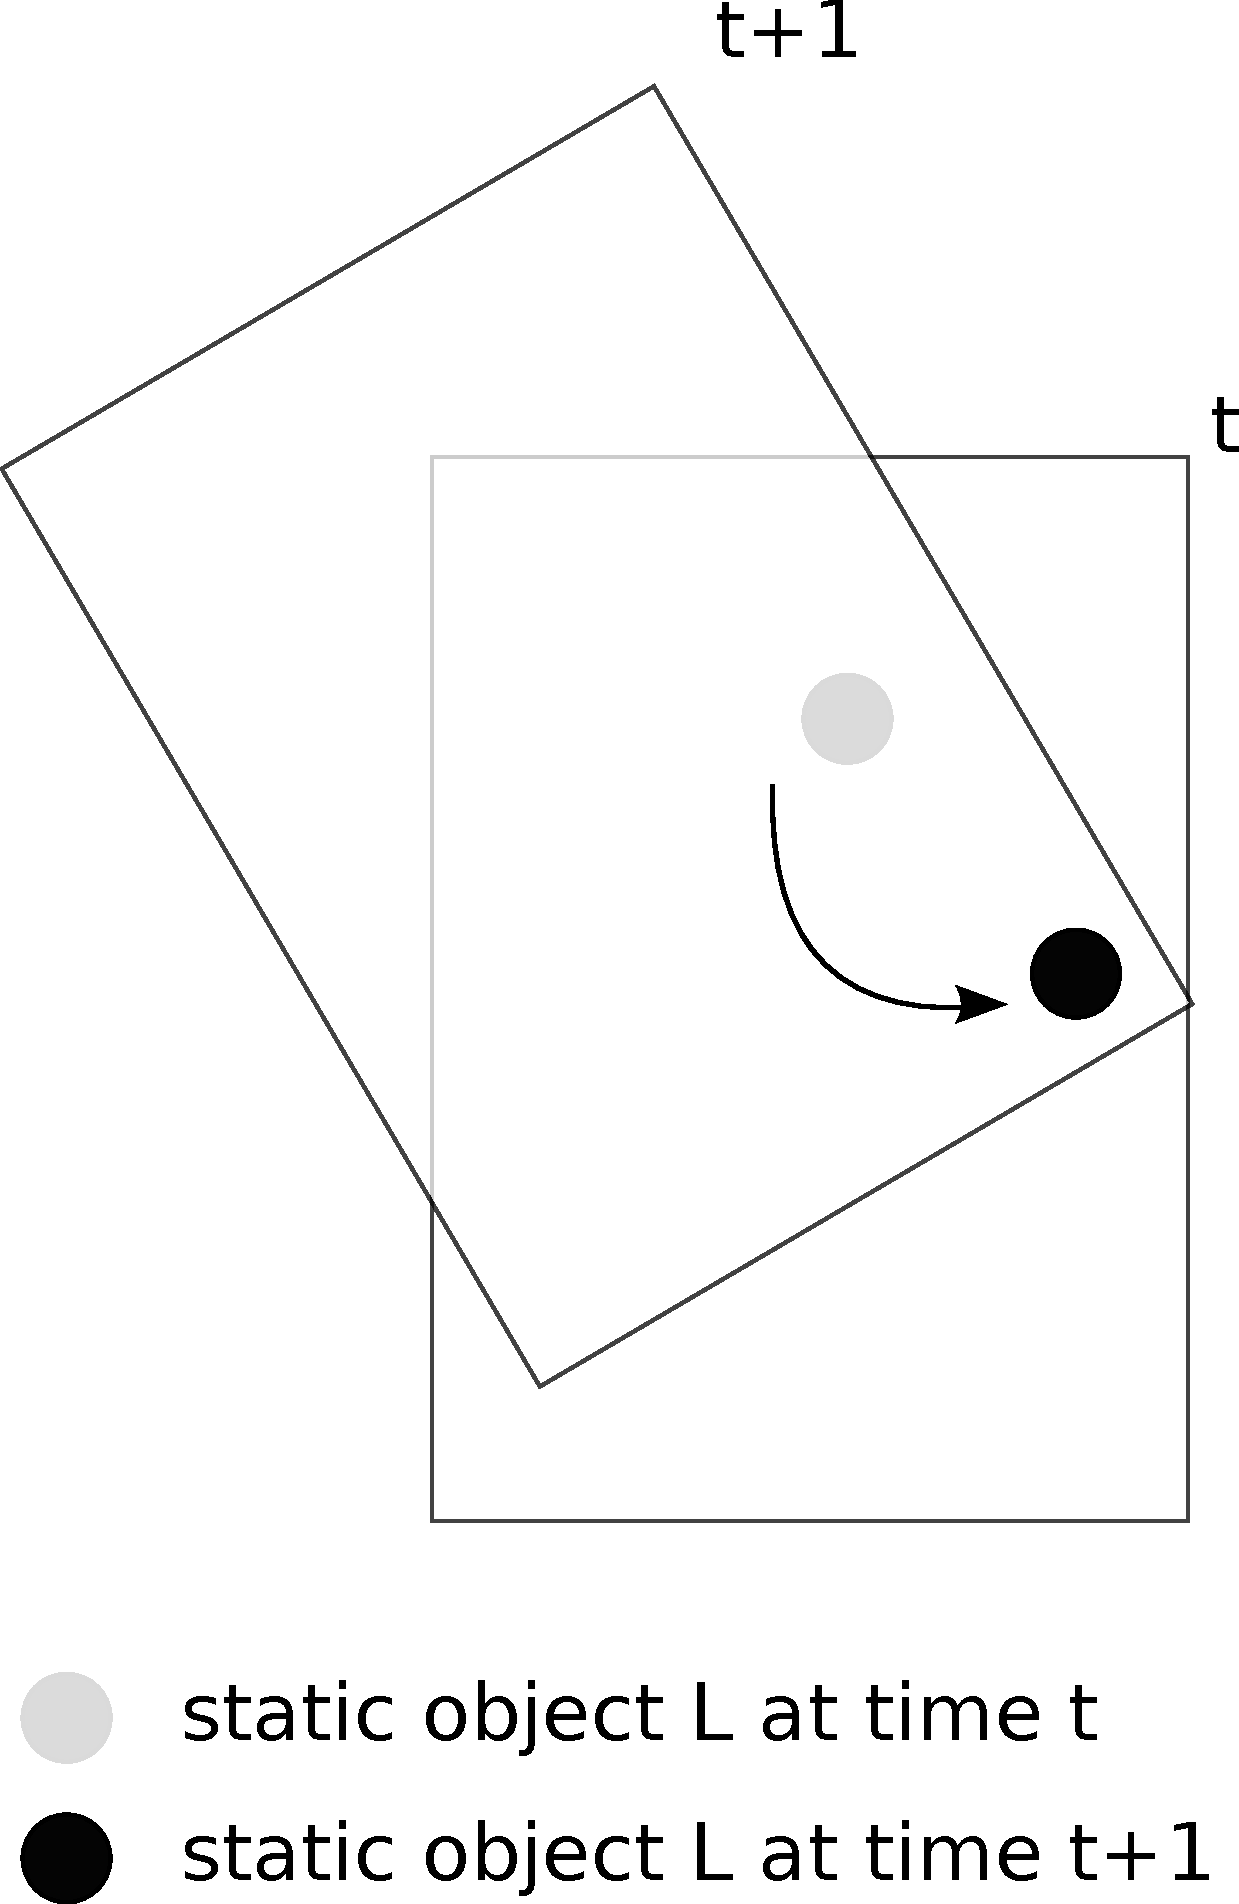
\includegraphics[width=0.3\columnwidth]{img/fig:motion:algorithm:nonstatic:02}

\begin{figure}[h]
   \centering
     \begin{tabular}{lr}
       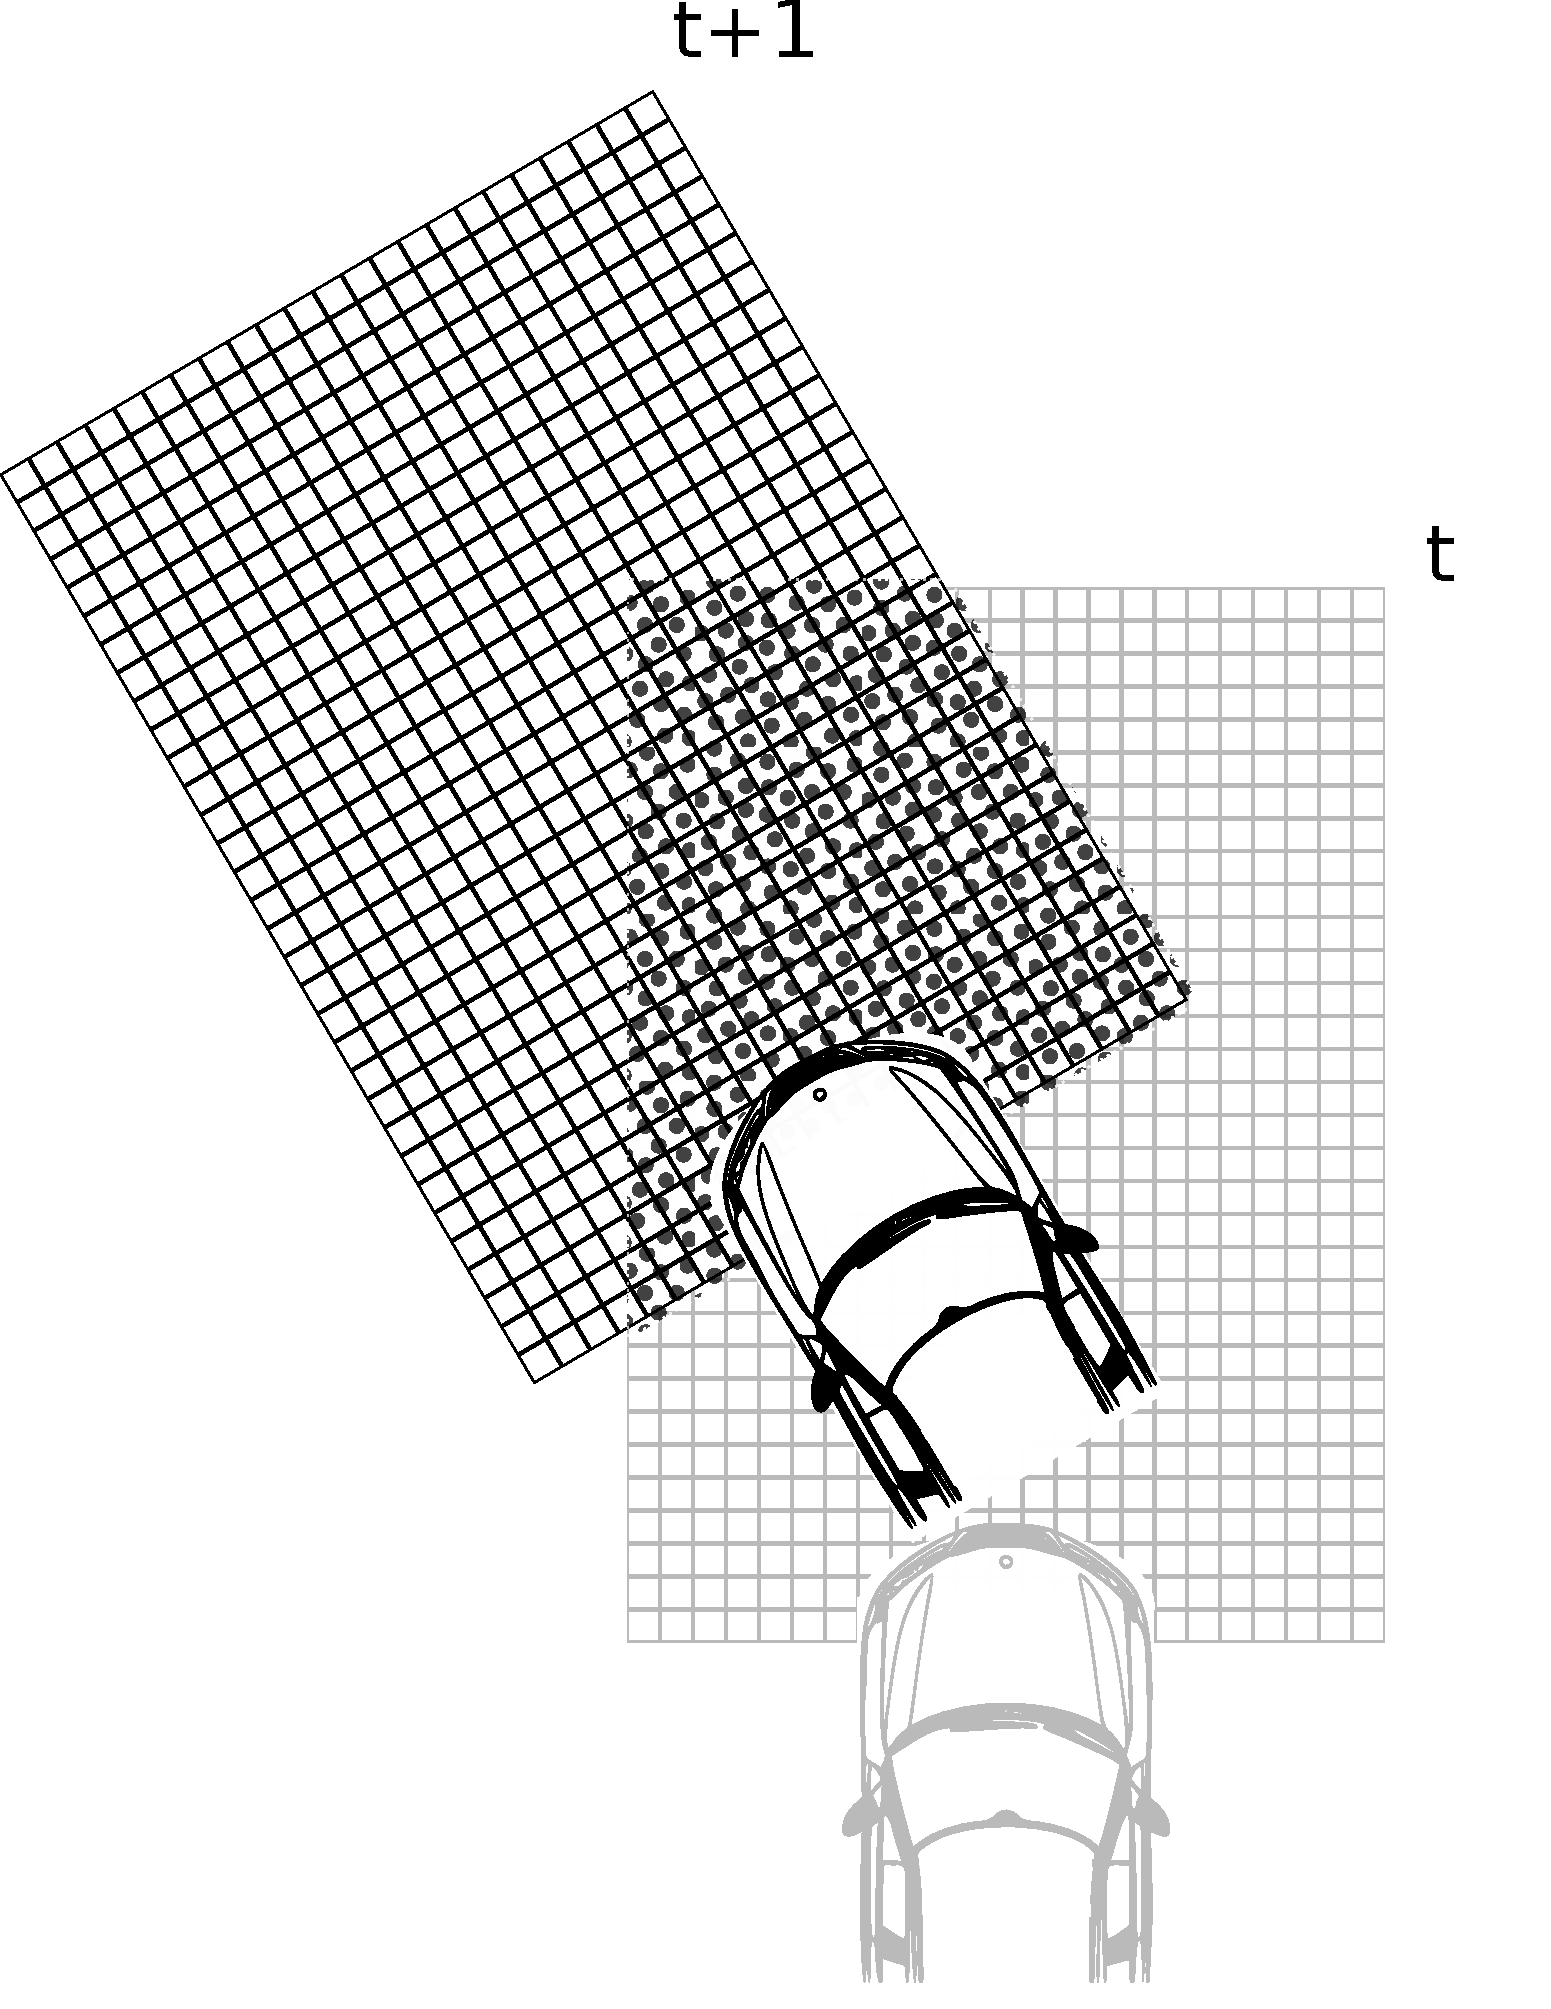
\includegraphics[width=0.35\columnwidth]{img/fig:motion:algorithm:nonstatic:01}
     \end{tabular}
   \caption{frames $f_t$ and $f_{t+1}$ with the intersection area}
   \label{fig:motion:algorithm:nonstatic:01}
 \end{figure}

The method developed in this document initially requires a static sensor, this constraint assumes that there is an exact correspondence between the cells among frames. Such constraint is not true in our application since the goal is to have it running in a moving vehicle, as an ADAS application. 

To better understand this issue take a look at the example: assume our vehicle is driving along a street and makes a left turn, we capture two frames, one while the car was driving straight $f_t$, and the second frame  after the car initiate the left turn $f_{t+1}$. We observe an a static object in the frame $f_t$ (\textit{e.g.} telephone pole in the sidewalk) that was located at $d_t$ meters from the car, and in the frame $f_{t+1}$ this very same object will be at $d_t-\Delta d(f_t,f_{t+1})$ and will be slightly moved to the right side (due to the left turn). The function $\Delta d$ returns the distance traveled by the car between the two frames. This behavior can be seen in the Figure~\ref{fig:motion:algorithm:nonstatic:01}, and as we can see, we can extract informations only from overlapping areas between two frames(Figure~\ref{fig:motion:algorithm:nonstatic:01} dotted area in the left image), but since this analysis is done in very small time variation, we have a great portion of overlapping area.

This problem is solved by introducing the Inertial Measurement Unit(IMU) data. The IMU provides information about the inertial behavior of the unit. Although not all information generated by the IMU are needed, the ones used are speed $s$, yaw angle, vertical $v_v$ and horizontal $v_h$ velocity. Those informations are used to apply the necessary transformation to the $f_t$ making its cells match the cells $f_{t+1}$. Thus finding the correspondence between cells of $f_t$ and $f_{t+1}$.

From the IMU information we calculate two parameters: angular velocity and the linear velocity. 

Angular velocity is obtained by finding the angle variation between the frames $f_t$ and $f_{t+1}$, according to the Equation~\ref{eq:angularvelocity}, $\Delta t$ represents the time variation between the frames.

\begin{equation}
\label{eq:angularvelocity}
\omega(f_t,f_{t+1}) = \frac{Yaw_{t+1}-Yaw_t}{\Delta t(f_t,f_{t+1})} 
\end{equation} 

The angular velocity is given in degrees, but the IMU gives us a quaternion for the angle of the vehicle. The quaternion is the most common way to represent angles in 3d world, due to the fast calculations and it solves the gym ball lock problem, which is common for euler angles. Converting the value from quaternion to Euler angles is straightforward by the Equation~\ref{eq:quaternion}.

\begin{equation}
\label{eq:quaternion}
Yaw=atan2(2(q_0 q_3+q_1 q_2),1-2(q_2^2+q_3^2))
\end{equation}

The angular velocity $\omega(f_t,f_{t+1})$ is used to adjust the angle of $f_t$, put this value aside, before apply this transformation to the frame $f_t$ we have to calculate the displacement of the grid.

At this point, we have the information about the proper angle for the frame $f_t$, the next step is to calculate the displacement of the frame. The displacement is calculated based on the actual velocity of the vehicle at the time $t$. 

The IMU keeps the velocity in two components, the horizontal $v_h$ and vertical $v_v$ velocities, and to obtain the actual velocity, we can apply the Equation~\ref{eq:velocity}, which extracts the velocity based on the two components.

\begin{equation}
\label{eq:velocity}
v_t=\sqrt{v_h^2+h_v^2}
\end{equation}

\subsection{Motion detection}
\label{ch03:motiondetection}

In this section we going to detail the technique that we developed to find moving parts of the environment. 

The input to this motion detection module consists of an occupancy grid and the vehicles velocities. The occupancy grid is generated by the fusion module described in previous section and that fuses data from eight layers of two laser scanners installed on the demonstrator vehicle. The vehicles velocities are provided by the MTi-G sensor unit.

Let us represent this occupancy grid at time $t$ as  $OG_t$. The value of each cell of this grid is between 0 and 1 i.e. $0 \leq OG_t[i] \leq 1$ (where $0 \leq i<N$ with $N$ being the total cells of this occupancy grid) which represents internal belief of the ego vehicle about the occupancy state of each cell where 0 means empty and 1 means occupied.

%explain XSens MTI-G in the beginning LIDAR, SENSOR MTI

The output of the \textit{XSens MTI-G} sensor, at time instant $t$,
consists of (along with other information) two components of velocity $v_t=(v_x, v_y)$ and values of
quaternion components for orientation $Q_t=(q_0, q_1, q_2, q_3)$. From those information we calculate the
translational and rotational velocities are represented by the tuple $u_t=(\nu_t, \omega_t)$, the velocity is calculated according to the Equation~\ref{eq:ch03:velocities}.

\begin{equation}
\label{eq:ch03:velocities}
\nu_t = \sqrt{v_x^2+v_y^2}
\end{equation}

To calculate rotational velocity of the vehicle we calculate yaw angle of the vehicle from the quaternion
as demonstrated in the Equation~\ref{eq:quaternion:yaw}, the $Yaw$ will be given in radians.

\begin{equation}
Yaw = atan2(2(q_0 q_3+q_1 q_2),1-2(q_2^2+q_3^2))
\label{eq:quaternion:yaw}
\end{equation}

And if $\Delta t$ is the time difference between two data frames at time $t$ and $t-1$ then rotational speed $\omega$
at time $t$ is equal to the yaw rate given as:
\begin{equation}
\omega_t = \frac{Yaw_t-Yaw_{t-1}}{\Delta t}
\end{equation}

At each time instant $t$ these $OG_t$ and $u_t$ are input to the algorithm that consists of 
following steps.

\paragraph{Free and occupied counters arrays} for each new input occupancy grid $OG_t$ we 
create two parallel counter arrays, having the same size ($N$ cells) as $OG_t$. The first called $FreeCount_t$ and the other called $OccupiedCount_t$ to keep the count of the number of times that a cell has been observed free and number of times it has been observed occupied, respectively. These arrays are initialized from $OG_t$ as follows ( $\forall i$  . $0 \leq i<N$ ):

\begin{equation}
OccupiedCount_t[i] =  \begin{cases} 1, & \mbox{ if $OG_t[i] > 0.5$} \\
                       0, & \mbox{otherwise} \end{cases}
\end{equation}
and
\begin{equation}
FreeCount_t[i] = \begin{cases} 1, & \mbox{ if $OG_t[i] < 0.5$} \\
                       0, & \mbox{otherwise} \end{cases}
\end{equation}

\paragraph{Counts update from previous step} Suppose $FreeCount_{t-1}$ and  $OccupiedCount_{t-1}$ are the
updated counter arrays at time $t-1$ and we want to update new counters $FreeCount_t$ and $OccupiedCount_t$
from these old counts. Since vehicle has undergone a position change determined by $u_t=(\nu_t, \omega_t)$
so there is no direct correspondence between cells of two occupancy grids $OG_t$ and $OG_{t-1}$ and we
must find transformations that map a cell in  $OG_{t-1}$ to a cell in $OG_{t}$ using $u_t$. This situation is
shown in Figure \ref{fig:gridmove}, $OG_{t-1}$ has origin at $O_{t-1}$ and $OG_t$ has origin at $O_t$. To find this transformation suppose $O_{t-1}=(x_{t-1}, y_{t-1}, \theta_{t-1}) = (0,0,0)$ is the pose (position and orientation) of the occupancy grid at time instant $t-1$ (i.e in $OG_{t-1}$) and we want to find $O_t=(x_t, y_t, \theta_t)$, the pose of $OG_t$ with respect to $OG_{t-1}$ after it has undergone a motion of $u_t$. By taking $O_{t-1}=(0,0,0)$ in each iteration of the algorithm.

We highlight the fact that we solve localization only for two consecutives frames and do not care about the global localization. 

Now if $\Delta t$ is the time difference between the instants $t$ and $t-1$ then using circular motion model the pose $O_t$ is given as:

\begin{equation}
\left[\begin{array}{c}x_t \\ y_t\\ \theta_t \end{array} \right] = 
\left[\begin{array}{c} {\nu_t \over \omega_t} \sin(\omega_t \Delta t) \\ {\nu_t \over \omega_t} - {\nu_t \over \omega_t} \cos(\omega_t \Delta t) \\ \omega_t \Delta t \end{array}\right]
\end{equation}

\begin{figure}[h]
\begin{center}
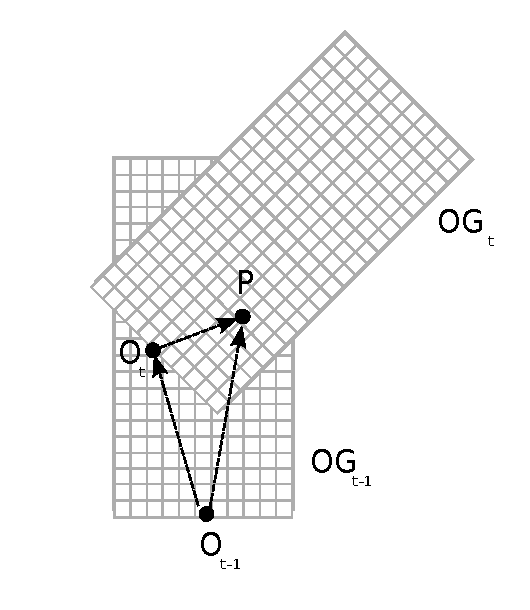
\includegraphics[scale=0.8]{img/fig:translation}
\caption{Position of the grid at instants $t-1$ and $t$. Vehicle undergoes a motion of $u_t=(\nu_t, \omega_t)$ to move from $O_{t-1}$ to $O_t$. We need to find the position of point $P$ of grid $OG_{t-1}$ in grid $OG_t$.}
\label{fig:gridmove}
\end{center}
\end{figure}

An important thing is to notice that we are concerned with the localization of two consecutive frames only
and need not solve the complete SLAM problem, making the technique very fast. Moreover, empirical observation suggests that the odometry error between two consective frames is less than 10 cm whereas the cell size assigned is $20cm \; x \; 20cm$ enabling us to assume that cell mapping (explained next) from grid at $t-1$ to grid at $t$ is exact.

Mapping a cell of the grid $OG_{t-1}$ to $OG_t$ consist in bring $OG_{t-1}$ up to speed based in the MTi-G sensor unit information. Suppose point $P$ (shown in Figure \ref{fig:gridmove}) is the center of a cell in grid $OG_{t-1}$ and we want to find its corresponding cell in grid $OG_t$. We define following two pose manipulation operations. if $P_{ij}=[x_{ij}, y_{ij}, \theta_{ij}]^T$ is the pose of origin $j$ w.r.t origin $i$ and $P_{jk}=[x_{jk}, y_{jk}, \theta_{jk}]^T$ is the pose of origin $k$ w.r.t $j$ then the pose of $k$ w.r.t $i$ denoted as $P_{ik}=[x_{ik}, y_{ik}, \theta_{ik}]^T$ is given as:

\begin{equation}
P_{ik} \equiv \oplus (P_{ij}, P_{jk}) = \left[ \begin{array}{c}
x_{jk}\cos(\theta_{ij})-y_{jk}\sin(\theta_{ij})+x_{ij} \\
x_{jk}\sin(\theta_{ij})+y_{jk}\cos(\theta_{ij})+y_{ij} \\
\theta_{ij}+\theta_{jk} \end{array} \right] 
\end{equation}

For the pose $P_{ij}$ the reverse pose relationship $P_{ji}=[x_{ji}, y_{ji}, \theta_{ji}]^T$ (pose of $i$ w.r.t $j$) is defined as:

\begin{equation}
P_{ji} \equiv \ominus (P_{ij}) = \left[ \begin{array}{c}
-x_{ij}\cos(\theta_{ij})-y_{ij}\sin(\theta_{ij}) \\
x_{ij}\sin(\theta_{ij})-y_{ij}\cos(\theta_{ij}) \\
-\theta_{ij} \end{array} \right] 
\end{equation}

Since the pose of $O_t$ w.r.t $O_{t-1}$ is $P_{O_{t-1}O_t}=[x_t,y_t,\theta_t]^T$ and point $P$ has pose $P_{O_{t-1}P}=[x,y,0]^T$ w.r.t $O_{t-1}$. The pose of this point $P$ w.r.t $O_t$ is calculated as:

\begin{equation}
P_{O_tP} = \oplus (P_{O_tO_{t-1}}, P_{O_{t-1}P})
\end{equation}

or

\begin{equation}
P_{O_tP} = \oplus (\ominus(P_{O_{t-1}O_t}), P_{O_{t-1}P})
\end{equation}

First two components of $P_{O_tP}$ give $x$ and $y$ position of the point $P$ w.r.t origin $O_t$. From these $x$ and $y$ values we can easily calculate the index of the cell where point $P$ lies in grid $OG_t$. In the Equation~\ref{eq:grid:cell:calculation} we calculate the row and column of the cell in which $P$ lies, where $cell_{size}$ is $0.2m$ and $gridWidth$ is $20m$ .

\begin{equation}
cell(column,row)=\left\{\frac{1}{cell_{size}}(x+\frac{gridWidth}{2}),\frac{y}{cell_{size}} \right\}
\label{eq:grid:cell:calculation}
\end{equation}


%\begin{equation}
%cell_{column}=(x+gridWidth/2)/cellSize
%\end{equation}

%\begin{equation}
%cell_{row}=y/cellSize
%\end{equation}

These transformations will map a cell having index $i$ in $OG_{t-1}$ to a cell having index $j$ in grid $OG_t$. If this cell $j$ is visible in $OG_t$ i.e $0 \leq j<N$ then we can update new count values for this cell as follows:

\begin{equation}
FreeCount_t[j] = FreeCount_t[j] + FreeCount_{t-1}[i]
\end{equation}

and

\begin{equation}
OccupiedCount_t[j] = OccupiedCount_t[j] + OccupiedCount_{t-1}[i]
\end{equation}

We repeat this process for all cells of grid $OG_{t-1}$ to update counter values in grid $OG_{t}$.

\paragraph{Motion detection} After the counts arrays have been updated as explained above the motion grid can be calculated from the new data as follows:

\begin{equation}
MotionGrid_t[i] = \begin{cases} 1, & \mbox{$OG_t[i] > 0.5$ and} \\ & \mbox {$FreeCount_t[i]>2\;  x \; OccupiedCount_t[i]$} \\
                                0, & \mbox{otherwise}\end{cases}
\end{equation}
After this process, the $MotionGrid_t$ becomes a binary grid, where it has 1's assigned to the cells which belongs to moving parts, and 0's otherwise.

%%%%%%%%%%%%%%%%%%%%%%%%%%%%%%%%%%%%%%%%%%%%%%%%%%%%%%%%%%%%%%%%%%%%%%%%%%%%%%%%



%\subsection{Solution}


%\section{summary}

%summary